\section{Discussion}
\label{sec:discussion}

In the previous section, we have validated the Refusal Index with its analytical model and experimental results, showing that the RI uniquely and consistently evaluates the knowledge-aware refusal ability. 
In this section, we provide insights into LLM factuality through the lens of Refusal Index. 
Our interpretable and practical method provides several new insights into model calibration that were previously obscured by heuristic metrics. 



\paragraph{Does prompting models to be more cautious mitigate miscalibration?} LLMs are notorious for their overconfidence; by default, LLMs will try to answer all questions beyond their knowledge. 
One might wonder whether instructing models to reduce confidence helps with this problem. 
Our proposed RI gives a more holistic understanding to this question. 
As shown in Table~\ref{tab:qwen25_simpleqa_prompt_strategies}, while increasing refusal rates increases the correct answer rate in answered questions (increasing C/A), their RI remains stable and far from perfection. 
This means that even when a model shows the same refusal rate as its error rate (no system bias), there still remains a gap from perfect refusal decisions (perfect alignment between refusal and error). 
In other words, RI indicates and quantifies this gap independent of specific refusal rates from the model.

\paragraph{What factors lead to better knowledge-aware refusal?}

\begin{wrapfigure}{r}{0.5\textwidth}
    \centering
    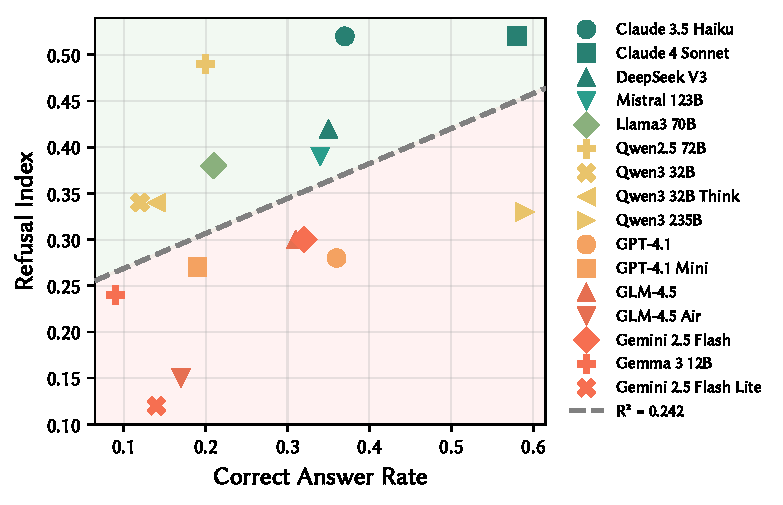
\includegraphics[width=0.45\textwidth]{Figures/simpleqa_refusal_vs_accuracy_scatter.pdf}
    \caption{Scatter plot of Refusal Index vs. Correct Answer Rate.}
    \label{fig:simpleqa_refusal_vs_accuracy_scatter}
\end{wrapfigure}

Naturally, we are curious about what factors in LLM designs have the most impact on RI. 
Within the model scope covered in our test, we didn't find high correlation between RI and model parameter sizes, accuracy, or refusal rates. 
We plot the relationship between correct answer rate in SimpleQA under normal refusal rates and their average RI, as shown in the scatter plot in \Figref{fig:simpleqa_refusal_vs_accuracy_scatter}. 
The correct answer rate shows a mere $R^2=0.235$ correlation to Refusal Index, suggesting higher model accuracy at factual tasks does not necessarily lead to more knowledge-aware refusals. 
Interestingly, we find \emph{model family} is a strong predictor of RI. 
In our experiments, models from \emph{Claude} and \emph{Qwen} (except Qwen 235B) are well above the regression line, showing above-average knowledge-aware refusal abilities. 
In contrast, all models from \emph{Gemini}, \emph{GPT-4.1} and \emph{GLM-4.5} are below the regression line. 
Especially \emph{Claude} models show the highest RI on both Claude-3.5 Haiku and Claude-3.5 Sonnet. 
These findings hint that the specific training pipeline and data distribution used by different model providers might play a more important role in the knowledge-aware refusals.

\begin{wraptable}{r}{0.6\textwidth}
    \vspace{-\baselineskip}
    \centering
    \caption{Refusal Index results on hallucination benchmarks.}
    \label{tab:hallu_model_comparison}
    \resizebox{\linewidth}{!}{%
    \begin{tabular}{l c c c c}
    \toprule
    \multirow{3}{*}{\textbf{Model}} & \multicolumn{2}{c}{\textbf{Truth Available}} & \multicolumn{2}{c}{\textbf{Truth Unavailable}} \\
    \cmidrule(lr){2-3} \cmidrule(lr){4-5}
    & \textbf{Precise-} & \textbf{Counter-} & \textbf{Incon-} & \textbf{Unans-} \\
    & \textbf{Wiki} & \textbf{factual} & \textbf{sistency} & \textbf{werable} \\
    \midrule
    Gemma-3-12b & 0.36 & 0.56 & 0.22 & 0.12 \\
    Qwen3-32B & 0.48 & 0.60 & 0.27 & 0.24 \\
    Qwen2.5-72B & \textbf{0.54} & 0.56 & 0.22 & 0.40 \\
    Llama-3.1-70B & 0.52 & \textbf{0.70} & 0.17 & 0.31 \\
    Mistral-Large & 0.50 & 0.38 & \textbf{0.34} & \textbf{0.52} \\
    \midrule
    Average & 0.48 & 0.56 & 0.24 & 0.32 \\
    \bottomrule
    \end{tabular}%
    }
    \vspace{-0.5em}

\end{wraptable}

\paragraph{Is a model's refusal ability affected by context?} 
We further expand RI to a more realistic setting where models generate answers conditioned on grounding context. 
In Table~\ref{tab:hallu_model_comparison}, each dataset tests model refusal ability in different scenarios:
\textbf{PreciseWiki} requires models to recall information from training data; 
\textbf{Counterfactual} tests models' ability to refrain from hallucinating from misleading and counterfactual context (e.g., the moon is made of cheese). 
\textbf{Inconsistency} and \textbf{Unanswerable} test if models refuse when answers are not available, where \textbf{Inconsistency} provides conflicting information and \textbf{Unanswerable} does not provide answers in context.
Results show that RI values for PreciseWiki are similar to those of SimpleQA, and models generally have good ability to identify and avoid counterfactual context. However, when ground truth becomes unavailable, models are showing much worse knowledge-aware refusal. 
This suggests that models' knowledge-aware refusal may rely on existing partial information on the answer; they make poorer knowledge-aware refusals when the answer never appears in training data or context.

\paragraph{Limitations of RI.}
While the Refusal Index is a useful metric for measuring knowledge-aware refusal, there are limitations that practitioners should be aware of. 
First, as the two-pass evaluation requires instructing the model to either refuse or provide forced answers, it requires a relatively capable model. 
Second, our formulation and validation of RI are focused on \emph{knowledge-aware refusal}, which may not hold for other kinds of refusals, such as refusals for safety reasons. 
Finally, from both the definition and experimental results, knowledge-aware refusal is a relatively weak signal compared to other metrics like correct answer rate. 
Thus, we recommend using larger datasets in evaluation to obtain a more stable RI score. 
Nevertheless, RI provides a pragmatic metric for knowledge-aware refusal, which is important but overlooked by previous metrics.